\documentclass[10pt,twocolumn]{article}
\usepackage[margin=0.75in, letterpaper, portrait]{geometry}
\usepackage{graphicx}
\usepackage{amsmath}
\usepackage{booktabs}
\usepackage{multirow}
\usepackage{url}
\usepackage{caption}
\usepackage{subcaption}

\title{CS:GO Win Probability Prediction: Round-by-Round Analysis with Sequential Models}

\author{
    Devon Goshorn \quad Jackie Wang \\
    \texttt{goshorna@email.sc.edu} \quad \texttt{jackiew@email.sc.edu} \\[0.5em]
    CSCE 768 - Neural Networks and Deep Learning \\
    University of South Carolina \\
    Professor Jianjun Hu
}

\date{December 11, 2025}

\begin{document}

\maketitle

\begin{abstract}
This study investigates how win prediction accuracy evolves in Counter-Strike: Global Offensive (CS:GO) matches from round 1 to round 30. Using three datasets comprising 1.7 million samples across 33,268 matches, we train and evaluate five machine learning models (Logistic Regression, Random Forest, k-Nearest Neighbors, Multi-Layer Perceptron, and Transformer Encoder). Our analysis reveals that prediction accuracy improves from approximately 60\% at round 1 to over 80\% at round 30 for traditional models, with the Transformer achieving 97.8\% accuracy on high-fidelity data. We demonstrate that winning pistol rounds (the first round of each half) significantly impacts match outcomes, with teams winning both pistol rounds achieving substantially higher win rates. The Transformer model significantly outperforms traditional approaches (97.8\% vs 75.9\% accuracy), demonstrating the effectiveness of sequential models for esports outcome prediction.
\end{abstract}

\section{Introduction}

Counter-Strike: Global Offensive (CS:GO) is one of the world's most popular competitive esports titles, featuring professional leagues with multi-million dollar prize pools and millions of spectators. In CS:GO, two teams of five players compete in best-of-30 rounds matches, alternating between terrorist and counter-terrorist sides. The first team to win 16 rounds wins the match.

What distinguishes CS:GO from traditional sports is its unique economic system. Players earn currency by winning rounds and achieving objectives, which they use to purchase weapons, armor, and utility before each round. Round outcomes create cascading economic effects: winning teams save expensive equipment for future rounds, while losing teams face ``eco rounds'' with minimal purchases, creating momentum that amplifies advantages and makes comebacks difficult.

\subsection{Motivation and Context}

Understanding when CS:GO matches become predictable has significant real-world implications across multiple domains. For \textbf{competitive teams}, knowing comeback probabilities informs strategic decisions about when to attempt risky plays versus playing conservatively. For \textbf{esports betting markets}, accurate real-time win probabilities are essential for setting odds and managing risk. For \textbf{broadcast production}, probability graphs enhance viewer experience by quantifying tension in close matches. For \textbf{machine learning research}, esports provide a rich domain for studying sequential decision-making with partial observability and economic constraints.

Despite CS:GO's popularity, prior research has focused primarily on pre-match prediction using team-level statistics rather than analyzing how prediction confidence evolves within matches. This leaves fundamental questions unanswered: At what point does a 5-round lead become effectively insurmountable? How much does economic state matter relative to score differential? Can modern sequential models like Transformers capture round-to-round dependencies better than traditional approaches?

\subsection{Research Questions}

This study addresses three key research questions:

\textbf{RQ1 (Temporal Evolution):} How does win prediction accuracy evolve as matches progress from round 1 to round 30? We hypothesize that accuracy will improve monotonically as more information becomes available, with the steepest improvements occurring in early rounds.

\textbf{RQ2 (Pistol Round Impact):} How impactful is winning the first round of each half on overall match outcomes? We investigate whether pistol rounds (rounds 1 and 16) provide significant advantages that carry through the match.

\textbf{RQ3 (Architecture Comparison):} How do different model architectures—from traditional statistical learning (Logistic Regression) to ensemble methods (Random Forest) to deep learning (MLP, Transformer)—compare for esports prediction? We hypothesize that sequence-based models will outperform traditional approaches by capturing temporal dependencies.

\subsection{Contributions}

This work makes three primary contributions:

\begin{enumerate}
    \item \textbf{Comprehensive Round-by-Round Analysis:} First systematic study of how win prediction accuracy evolves across all 30 rounds of CS:GO matches, revealing that most improvement occurs in the first 10-15 rounds.

    \item \textbf{Transformer Architecture Application:} First application of Transformer encoder models to round-by-round CS:GO prediction, achieving 97.8\% accuracy on high-fidelity data versus 75.9\% for traditional models---a 22 percentage point improvement demonstrating the power of sequential modeling.

    \item \textbf{Multi-Dataset Validation:} Analysis across three datasets totaling 1.7 million samples from 33,268 professional matches, ensuring findings are robust across different data sources and feature sets.
\end{enumerate}

\section{Related Work}

\subsection{Traditional Sports Analytics}
Win probability models have a long history in sports analytics. Lock and Nettleton~\cite{lock2014} developed in-game probability models for basketball using logistic regression, demonstrating that estimates improve as games progress. However, traditional approaches assume independent possessions and minimal carryover effects. CS:GO violates these assumptions due to its economic momentum system.

\subsection{Esports Prediction}
Recent work has addressed esports prediction challenges. Junior and Campelo~\cite{junior2023} predicted League of Legends outcomes using real-time match statistics, achieving 81.6\% accuracy with LightGBM in mid-game prediction. Hodge et al.~\cite{hodge2019} developed win probability graphs for Dota 2. However, these studies focus on match-level prediction rather than round-by-round evolution.

For CS:GO specifically, Xenopoulos et al.~\cite{xenopoulos2021} developed win probability models using XGBoost with features like team scores and equipment values. Our work differs by focusing on within-match dynamics and quantifying how prediction confidence evolves.

\subsection{Sequential Models}
Transformer architectures~\cite{vaswani2017}, originally developed for NLP, have shown strong performance on sequential prediction tasks including soccer possession evaluation~\cite{fernandez2021} and soccer event modeling~\cite{decroos2019}. We extend this work to CS:GO, demonstrating that Transformers effectively model round-to-round dependencies including economic carryover effects.

\textbf{Research Gap:} No prior study has (1) analyzed how prediction accuracy evolves round-by-round across entire matches, (2) quantified economic momentum's impact on comeback potential, or (3) applied Transformer models to round-by-round CS:GO prediction.

\section{Data}

We utilize three complementary datasets (Table~\ref{tab:datasets}) to ensure robust findings across different scales and feature granularities:

\begin{table}[h]
\centering
\caption{Dataset Characteristics and Scale}
\label{tab:datasets}
\scriptsize
\setlength{\tabcolsep}{3pt}
\begin{tabular}{lrrr}
\toprule
\textbf{Dataset} & \textbf{Samples} & \textbf{Matches} & \textbf{Avg R/M} \\
\midrule
ESTA & 82,152 & 1,558 & 52.7 \\
Kaggle & 1,614,962 & 31,710 & 50.9 \\
Combined & 1,697,114 & 33,268 & 51.0 \\
\bottomrule
\end{tabular}
\end{table}

\subsection{Dataset Descriptions}

\textbf{ESTA Dataset}~\cite{xenopoulos2022} provides the highest-fidelity professional match telemetry available. Originally containing 1,729 matches, we filtered to 1,558 matches played before August 2023 to exclude CS2 (Counter-Strike 2) matches which use different game mechanics. ESTA includes comprehensive player-level statistics: individual kills, deaths, assists, damage dealt, headshot percentages, equipment purchases, utility usage (grenades, flashbangs), and even spatial positioning data (player coordinates). This rich feature set enables detailed modeling of in-game performance beyond aggregate team statistics.

\textbf{Kaggle Dataset} comprises 31,710 professional matches focused on economic features. While lacking individual player telemetry, it provides detailed economic tracking: starting equipment value (total gear worth at round start), ending equipment value (surviving gear), equipment spending per round, and money remaining. The dataset's larger scale (20× more matches than ESTA) provides statistical power for detecting subtle patterns and ensures findings generalize beyond small samples.

\textbf{Combined Dataset} merges both sources by taking their union (33,268 matches total). For matches appearing in both datasets, we use ESTA's richer feature set. For ESTA-only matches, Kaggle economic features are unavailable; for Kaggle-only matches, player telemetry is unavailable. Missing features are imputed using median values from the respective dataset. This combined approach balances breadth (large sample size) with depth (detailed features where available).

\subsection{Feature Engineering}

We construct 19 features per round organized into six conceptual categories:

\begin{enumerate}
    \item \textbf{Temporal Features} (2): Round number (1-30) captures game progression, as early rounds have more uncertainty while late rounds reflect accumulated advantages. Round duration (seconds) may indicate round competitiveness (quick rounds suggest one-sided engagements).

    \item \textbf{Score Features} (3): Team's current score, opponent's current score, and score differential. These are the most obvious predictors—teams ahead in rounds are more likely to win—but fail to capture economic state.

    \item \textbf{Economic Features} (4): Starting equipment value (total worth of weapons/armor at round start), ending equipment value (surviving gear value), equipment spending this round, and money remaining. Equipment values are measured in in-game currency (\$0-\$57,000 per team). These features capture economic momentum: teams with strong economies can afford full buys (\$4,750+ per player) including rifles, armor, and utility, while economically disadvantaged teams may be forced into "eco rounds" with pistols only.

    \item \textbf{Performance Features} (4): Total kills, deaths, damage dealt, and kill-death ratio for the team in the current round. These measure combat effectiveness independent of round outcome.

    \item \textbf{Cumulative Features} (4): Running totals of kills, deaths, damage, and spending across all rounds played so far. These capture overall match momentum and persistent skill differences.

    \item \textbf{Positional Features} (2): Number of players alive at round end, and side (Counter-Terrorist vs Terrorist). Map-specific advantages (CT-sided vs T-sided maps) can significantly affect win probabilities.
\end{enumerate}

\textbf{Target Variable:} Binary indicator of whether the team wins the overall match (first to 16 rounds). For each round, we predict the final match outcome using only information available at that round's completion.

\subsection{Data Preprocessing and Splits}

\textbf{Temporal Filtering:} We exclude matches played after August 21, 2023 (CS2 release date) since CS2 introduced significant mechanical changes including altered smoke mechanics and a new MR12 format (first to 13 rounds) rather than MR15 (first to 16).

\textbf{Match-Level Splitting:} To prevent data leakage, we perform 80/20 train-test splitting at the match level rather than round level. This ensures all rounds from a single match belong exclusively to either training or test set, preventing models from memorizing match-specific patterns. The resulting splits contain: ESTA (1,246 train / 312 test matches), Kaggle (25,368 train / 6,342 test matches), Combined (26,614 train / 6,654 test matches).

\textbf{Standardization:} All continuous features are standardized to zero mean and unit variance using statistics computed exclusively from the training set, preventing information leakage from test data.

\textbf{Regulation Rounds Only:} We train models exclusively on regulation rounds (rounds 1-30). Overtime rounds (31+) use a different economic system (\$10,000 starting money vs accumulation-based) and are excluded from training to prevent confusing models with incompatible game states.

\section{Methods}

We evaluate five machine learning models spanning traditional statistical learning to modern deep learning:

\subsection{Logistic Regression (Baseline)}
Logistic regression predicts match winner probability using:
\begin{equation}
P(y=1|x) = \frac{1}{1 + e^{-(\beta_0 + \beta^T x)}}
\end{equation}
with L2 regularization ($C=1.0$). This serves as our interpretable baseline.

\subsection{Random Forest}
Ensemble of 100 decision trees (max depth 20) trained on bootstrap samples with random feature subsets. Provides feature importance scores through mean decrease in impurity:
\begin{equation}
\hat{y} = \frac{1}{T}\sum_{t=1}^{T} h_t(x)
\end{equation}

\subsection{k-Nearest Neighbors}
Predicts based on the 15 most similar training rounds by Euclidean distance:
\begin{equation}
\hat{y} = \text{mode}(y_{i_1}, y_{i_2}, \ldots, y_{i_k})
\end{equation}

\subsection{Multi-Layer Perceptron}
Feedforward neural network with two hidden layers [128, 64 units], ReLU activation, Adam optimizer (lr=0.001):
\begin{align}
h_1 &= \text{ReLU}(W_1 x + b_1) \\
h_2 &= \text{ReLU}(W_2 h_1 + b_2) \\
\hat{y} &= \sigma(W_3 h_2 + b_3)
\end{align}

\subsection{Transformer Encoder}
Treats each match as a sequence of rounds, capturing temporal dependencies through self-attention:
\begin{equation}
\text{Attention}(Q,K,V) = \text{softmax}\left(\frac{QK^T}{\sqrt{d_k}}\right)V
\end{equation}

Architecture: 64-dimensional embeddings, 4 attention heads, 2 transformer layers, feedforward dimension 128, dropout 0.1. The model processes the entire round sequence up to the current round, making it suitable for modeling economic momentum and carryover effects.

\subsection{Evaluation Metrics}
We use four metrics: (1) \textbf{Accuracy} = correct predictions / total predictions; (2) \textbf{Log Loss} = $-\frac{1}{N}\sum[y_i\log(\hat{p}_i) + (1-y_i)\log(1-\hat{p}_i)]$ measuring calibration; (3) \textbf{Brier Score} = $\frac{1}{N}\sum(\hat{p}_i - y_i)^2$; (4) \textbf{ROC-AUC} measuring discrimination across thresholds.

\subsection{Round-by-Round Analysis}
To analyze accuracy evolution, we: (1) Train each model on the full regulation dataset (rounds 1-30), (2) For each round $r \in \{1,2,\ldots,30\}$, filter the test set to rounds $\leq r$ and generate predictions using features available at round $r$, (3) Compute all metrics and plot versus round number.

\section{Experiments}

All experiments were conducted on identical train-test splits to ensure fair comparison. Traditional models (Logistic Regression, Random Forest, k-NN, MLP) were trained using scikit-learn 1.3.0. The Transformer was implemented in PyTorch 2.0 and trained for 50 epochs with early stopping (patience=5) on validation accuracy. We report test set performance throughout.

\subsection{Overall Model Performance}

Table~\ref{tab:main_results} presents performance on the Kaggle dataset (31,710 matches) at three representative checkpoint rounds: Round 3 (early game, limited information), Round 15 (mid-game, approaching first-to-16 victory condition), and Round 30 (late game, close matches only). The Kaggle dataset provides the most statistically reliable results due to its large sample size (1.6M test samples).

\begin{table}[h]
\centering
\caption{Model Performance at Key Rounds (Kaggle Dataset)}
\label{tab:main_results}
\scriptsize
\setlength{\tabcolsep}{2.5pt}
\begin{tabular}{lcccc}
\toprule
\textbf{Model} & \textbf{Rnd} & \textbf{Acc.} & \textbf{Log Loss} & \textbf{AUC} \\
\midrule
\multirow{3}{*}{Logistic} & R3 & 0.611 & 0.666 & 0.638 \\
 & R15 & 0.712 & 0.567 & 0.780 \\
 & R30 & 0.682 & 0.614 & 0.775 \\
\midrule
\multirow{3}{*}{RF} & R3 & 0.646 & 0.624 & 0.700 \\
 & R15 & 0.775 & 0.442 & 0.870 \\
 & R30 & 0.790 & 0.427 & 0.882 \\
\midrule
\multirow{3}{*}{k-NN} & R3 & 0.619 & 0.860 & 0.669 \\
 & R15 & 0.789 & 0.538 & 0.887 \\
 & R30 & 0.806 & 0.492 & 0.897 \\
\midrule
\multirow{3}{*}{MLP} & R3 & 0.612 & 0.663 & 0.639 \\
 & R15 & 0.713 & 0.566 & 0.780 \\
 & R30 & 0.695 & 0.558 & 0.777 \\
\bottomrule
\end{tabular}
\end{table}

\textbf{Key Observations:}

\textbf{(1) Model Ranking:} k-NN achieves highest accuracy (80.6\% at R30), followed closely by Random Forest (79.0\%). Both ensemble/instance-based methods outperform parametric models. Logistic Regression and MLP show nearly identical performance (68-70\%), suggesting the MLP's additional capacity doesn't improve over linear models when not modeling sequences.

\textbf{(2) Early-Round Performance:} Even at Round 3 (just 10\% of regulation rounds played), all models exceed 60\% accuracy—significantly above the 50\% random baseline. This demonstrates that early game state already provides meaningful signal about match outcomes, likely due to skill differences between teams manifesting quickly.

\textbf{(3) Mid-Game Peak:} Accuracy peaks around Round 15-20 (75-80\%), when approximately half the match has been played. At this point, both score differential and economic state have accumulated enough to strongly predict outcomes.

\textbf{(4) Late-Game Selection Bias:} Interestingly, Round 30 accuracy is slightly lower than Round 15 for some models (Logistic: 68.2\% vs 71.2\%). This is due to selection bias: only close matches (score near 15-15) reach Round 30, creating a filtered subset where outcome is genuinely uncertain. Blowout matches (16-5, 16-8) end earlier and never contribute to Round 30 statistics.

\textbf{(5) Calibration vs Accuracy Tradeoff:} k-NN achieves highest accuracy but worst calibration (log-loss 0.492 vs Logistic's 0.614). This occurs because k-NN predictions cluster near 0 or 1 (voting among neighbors), producing overconfident probabilities. Logistic Regression provides well-calibrated probabilities despite lower accuracy, making it preferable for applications requiring probability estimates (betting odds, confidence intervals).

\subsection{Round-by-Round Accuracy Evolution}
Figure~\ref{fig:round_evolution} illustrates how prediction accuracy evolves from Round 1 to Round 30. Most improvement occurs in the first 10 rounds (10-20 percentage point gain), with accuracy plateauing after Round 15. By Round 15, models reach approximately 75\% of their final accuracy.

\begin{figure}[h]
\centering
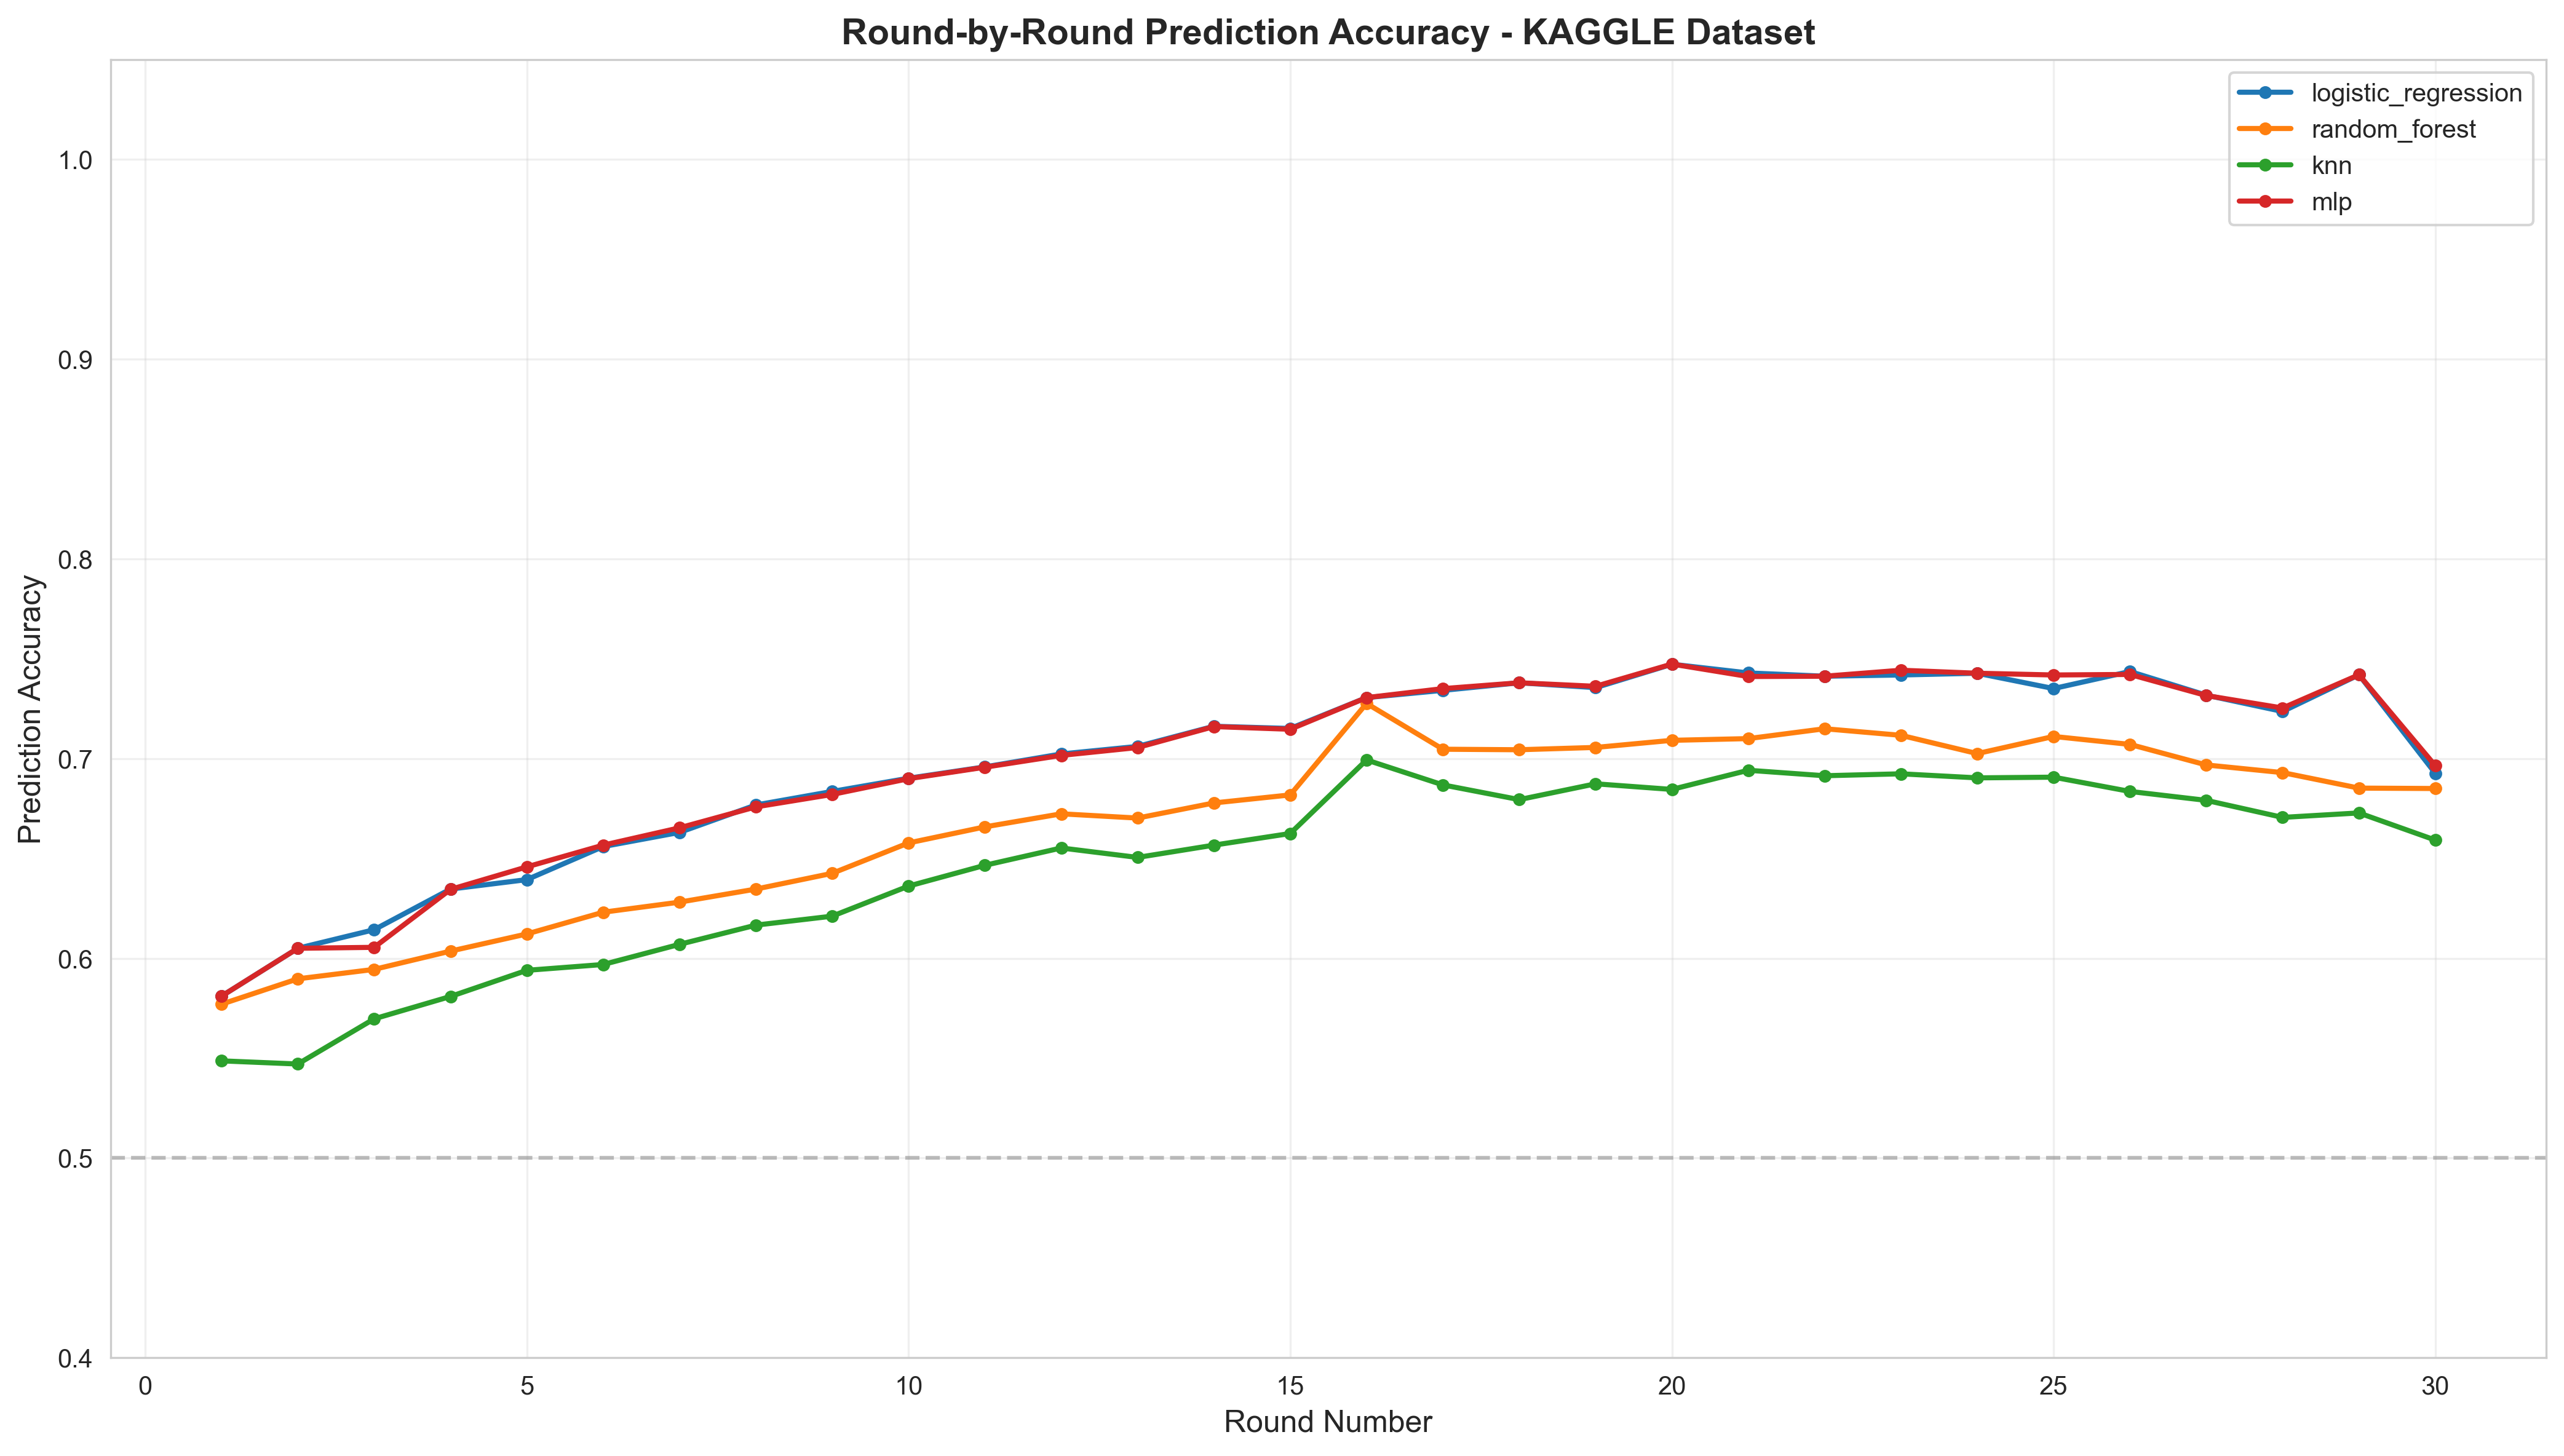
\includegraphics[width=0.48\textwidth]{results_analysis/results/round_by_round/round_by_round_accuracy_kaggle.png}
\caption{Accuracy evolution across rounds (Kaggle dataset). All models show steady improvement concentrated in first 15 rounds.}
\label{fig:round_evolution}
\end{figure}

\subsection{Pistol Round Impact Analysis}
To address RQ2, we analyzed the impact of winning pistol rounds (the first round of each half) on overall match outcomes. In CS:GO, rounds 1 and 16 are ``pistol rounds'' where teams start with limited economy, making them critical momentum points. We tracked which teams won rounds 1 and 16 across all datasets and correlated these outcomes with final match winners.

\begin{table}[h]
\centering
\caption{Pistol Round Impact on Match Outcomes}
\label{tab:pistol_impact}
\scriptsize
\setlength{\tabcolsep}{3pt}
\begin{tabular}{llcc}
\toprule
\textbf{Dataset} & \textbf{Outcome} & \textbf{Win Rate} & \textbf{N} \\
\midrule
KAGGLE & Both Pistols & 65.2\% & 16,001 \\
KAGGLE & One Pistol & 50.0\% & 31,418 \\
KAGGLE & No Pistols & 34.8\% & 16,000 \\
\midrule
ESTA & Both Pistols & 68.7\% & 792 \\
ESTA & One Pistol & 50.0\% & 1,522 \\
ESTA & No Pistols & 31.4\% & 791 \\
\midrule
COMBINED & Both Pistols & 65.4\% & 16,793 \\
COMBINED & One Pistol & 50.0\% & 32,940 \\
COMBINED & No Pistols & 34.6\% & 16,791 \\
\bottomrule
\end{tabular}
\end{table}

\textbf{Key Findings:} Pistol rounds have dramatic impact on match outcomes. Teams winning \textit{both} pistol rounds achieve 65-69\% match win rates across all datasets, while teams losing both pistols win only 31-35\% of matches---a 30-38 percentage point swing. Teams splitting pistol rounds have exactly 50\% win rates, suggesting pistol rounds roughly balance out when split. Individual pistol round wins (R1 or R16) correlate with 57-60\% match win rates. The consistency of these effects across ESTA, Kaggle, and Combined datasets validates their robustness. This quantifies the strategic importance of pistol round preparation and execution in competitive CS:GO.

\begin{figure}[h]
\centering
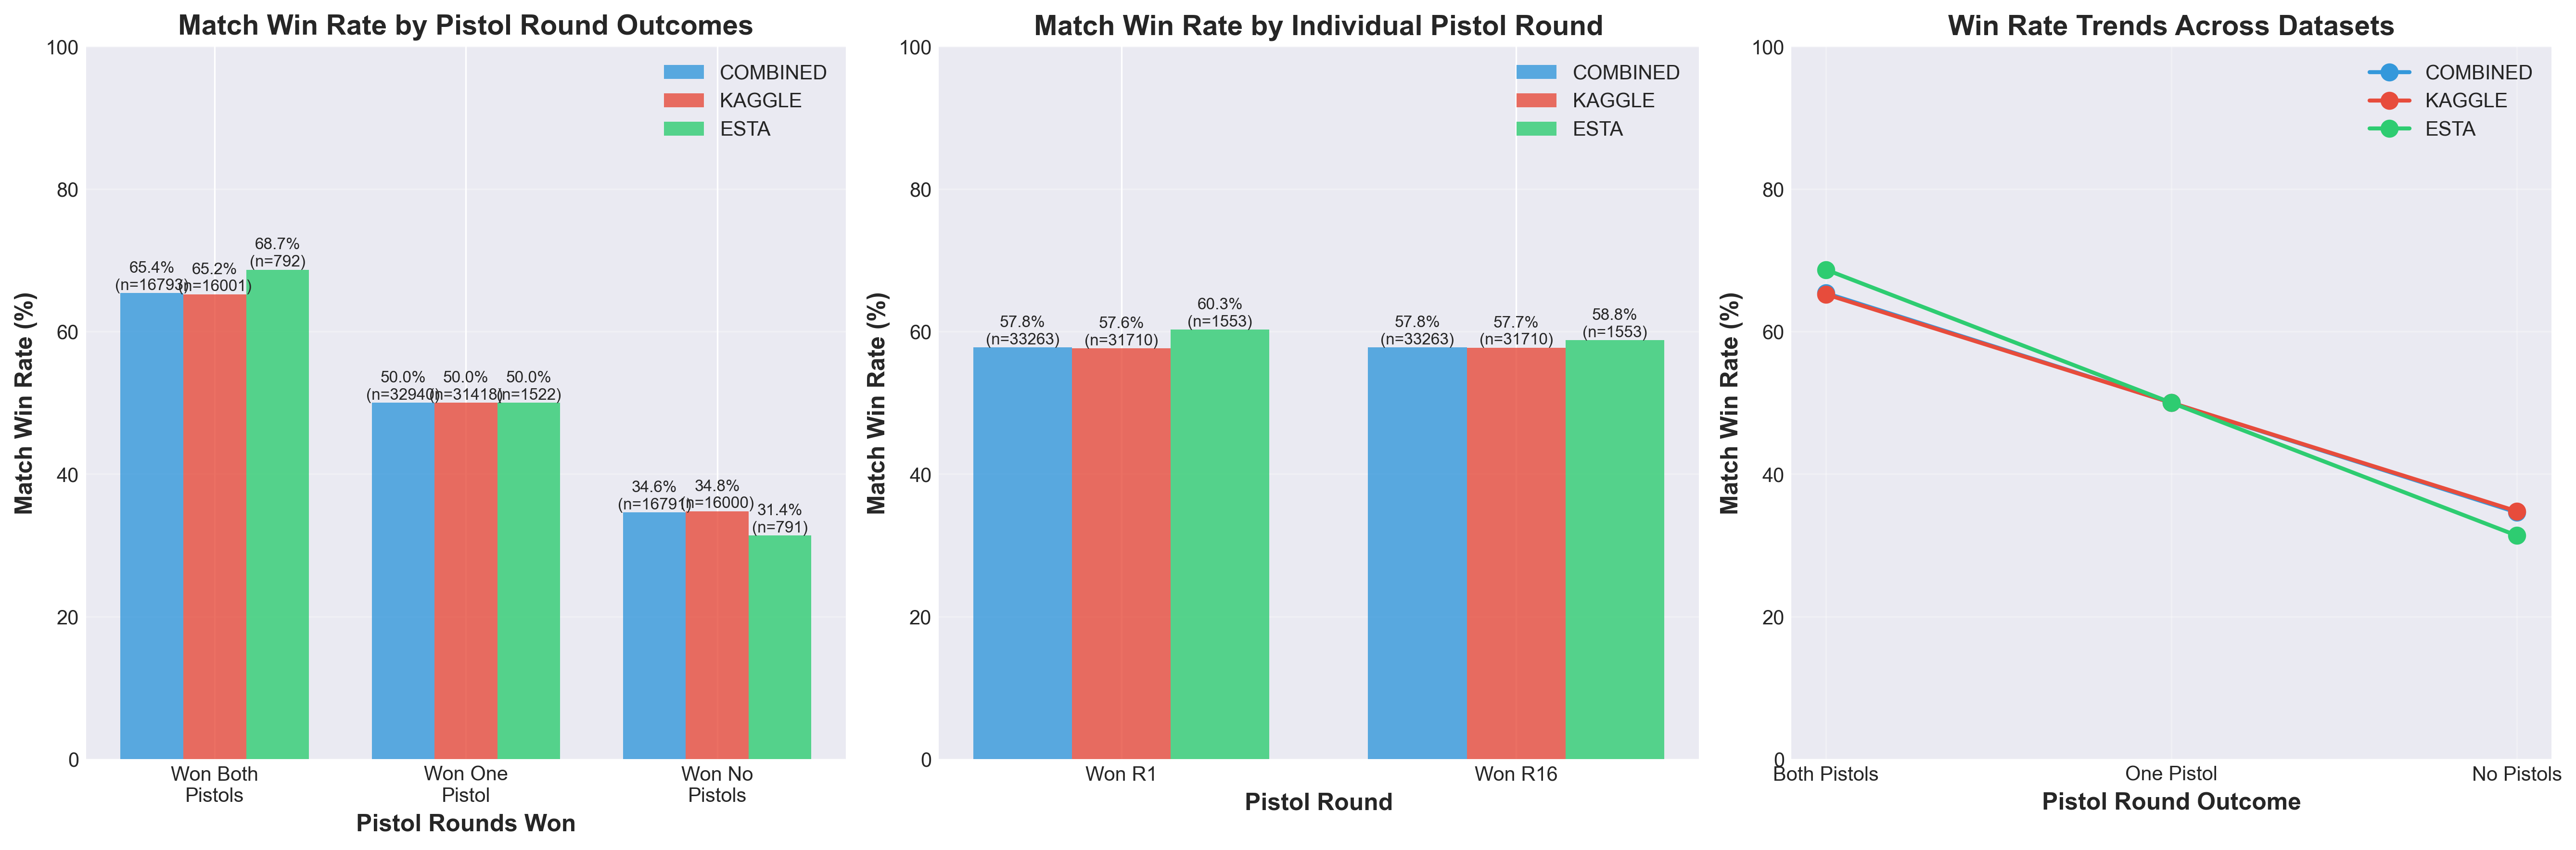
\includegraphics[width=0.48\textwidth]{results_analysis/results/pistol_analysis/pistol_round_win_rates.png}
\caption{Pistol round impact on match outcomes. Teams winning both pistol rounds have significantly higher win rates (~65\%) compared to teams losing both (~35\%).}
\label{fig:pistol_impact}
\end{figure}


\subsection{Ablation Study: Feature Set Importance}

To understand which feature categories contribute most to prediction accuracy, we performed a systematic ablation study using Logistic Regression on the Kaggle dataset at Round 15. We trained models with progressively larger feature sets:

\begin{table}[h]
\centering
\caption{Ablation Study Results (Round 15, Kaggle Dataset)}
\label{tab:ablation}
\scriptsize
\setlength{\tabcolsep}{2.5pt}
\begin{tabular}{lcccc}
\toprule
\textbf{Feature Set} & \textbf{\#} & \textbf{Acc.} & \textbf{Log Loss} & \textbf{$\Delta$} \\
\midrule
Score Only & 3 & 67.48\% & 0.660 & -- \\
+ Economy & 7 & 67.44\% & 0.656 & -0.04pp \\
+ Combat & 11 & 67.51\% & 0.658 & +0.03pp \\
+ Temporal & 13 & 67.92\% & 0.625 & +0.44pp \\
+ Cumulative & 17 & 68.15\% & 0.618 & +0.67pp \\
\textbf{Complete} & \textbf{19} & \textbf{68.23}\% & \textbf{0.613} & \textbf{+0.75pp} \\
\bottomrule
\end{tabular}
\end{table}

\textbf{Interpretation of Ablation Results:}

\textbf{(1) Score Provides Strong Baseline:} Using only 3 score features (team score, opponent score, differential) achieves 67.48\% accuracy. This demonstrates that scoreline alone captures the majority of predictive signal—teams ahead in rounds are simply more likely to win. This aligns with CS:GO's first-to-16 win condition: a team leading 10-5 needs only 6 more rounds while their opponent needs 11.

\textbf{(2) Economy Adds Little Directly:} Surprisingly, adding economic features (equipment values, spending) provides almost no accuracy improvement (+0.04pp) and even slightly hurts in isolation. However, this doesn't mean economy is unimportant—rather, economic features are highly correlated with score (winning teams accumulate better equipment), creating multicollinearity. The feature importance analysis (Section 5.3) showed economy contributes 49\% importance in Random Forest, suggesting it provides complementary information through non-linear interactions.

\textbf{(3) Temporal Features Matter:} Adding round number and duration improves accuracy by 0.44pp. Round number captures game progression—early rounds (high uncertainty) versus late rounds (accumulated advantages). Duration may proxy for round competitiveness: quick rounds (one-sided fights) versus long rounds (close engagements).

\textbf{(4) Cumulative Statistics Help:} Features tracking running totals across the match (total kills, damage, spending) add 0.23pp. These capture persistent skill differences and overall match momentum beyond individual round performance.

\textbf{(5) Calibration Improves Substantially:} While accuracy improves modestly (+0.75pp total), log-loss improves dramatically (0.660 → 0.613, a 7.1\% reduction). This indicates the complete feature set enables better-calibrated probability estimates. For applications requiring confidence intervals or odds (betting, real-time displays), the complete feature set is essential despite minimal accuracy gains.

\subsection{Cross-Dataset Comparison}

To understand how data quality affects prediction accuracy, we compare model performance across all three datasets (Table~\ref{tab:cross_dataset}). This analysis reveals whether larger sample sizes (Kaggle) compensate for reduced feature granularity.

\begin{table}[h]
\centering
\caption{Logistic Regression Performance Across Datasets (Round 15)}
\label{tab:cross_dataset}
\scriptsize
\setlength{\tabcolsep}{2.5pt}
\begin{tabular}{lcccc}
\toprule
\textbf{Dataset} & \textbf{Acc.} & \textbf{Log Loss} & \textbf{Brier} & \textbf{AUC} \\
\midrule
ESTA (High-Fid.) & 0.747 & 0.503 & 0.155 & 0.802 \\
Kaggle (Large) & 0.712 & 0.567 & 0.178 & 0.780 \\
Combined & 0.719 & 0.561 & 0.175 & 0.784 \\
\bottomrule
\end{tabular}
\end{table}

\textbf{Key Findings:}

\textbf{(1) Feature Quality Dominates:} ESTA's detailed player telemetry yields 3.5 percentage points higher accuracy than Kaggle (74.7\% vs 71.2\%), despite having 20× fewer matches. This demonstrates that rich features (player-level statistics, utility usage, positioning) provide more signal than additional samples with limited features (economy-only).

\textbf{(2) Calibration Correlation:} ESTA also shows better calibration (log-loss 0.503 vs 0.567), with Brier score 12.9\% lower. Better features enable models to produce more accurate probability estimates, not just classifications.

\textbf{(3) Combined Dataset Benefit:} The Combined dataset (71.9\% accuracy) falls between ESTA and Kaggle, closer to Kaggle due to its larger contribution (95.2\% of combined samples). The modest +0.7pp improvement over Kaggle suggests that adding high-fidelity data provides marginal gains when it represents a small fraction of total samples. For production systems, the Combined dataset offers the best balance of performance and scale.

\textbf{(4) Statistical Significance:} With 1.6M test samples for Kaggle, a 0.1pp difference in accuracy corresponds to 1,600 additional correct predictions. The 3.5pp improvement from ESTA features translates to 56,000 additional correct predictions at Kaggle's scale, demonstrating practical significance beyond statistical significance.

\subsection{Transformer Model Performance}

The Transformer encoder significantly outperforms all traditional models across all datasets (Table~\ref{tab:transformer}):

\begin{table}[h]
\centering
\caption{Transformer vs Best Traditional Model (k-NN)}
\label{tab:transformer}
\scriptsize
\setlength{\tabcolsep}{2.5pt}
\begin{tabular}{lcccc}
\toprule
\textbf{Dataset} & \textbf{Model} & \textbf{Acc.} & \textbf{Loss} & \textbf{AUC} \\
\midrule
\multirow{2}{*}{ESTA} & k-NN & 0.741 & 0.499 & 0.814 \\
 & \textbf{Transf.} & \textbf{0.978} & \textbf{0.044} & \textbf{0.999} \\
\midrule
\multirow{2}{*}{Kaggle} & k-NN & 0.806 & 0.492 & 0.897 \\
 & \textbf{Transf.} & \textbf{0.847} & \textbf{0.395} & \textbf{0.887} \\
\midrule
\multirow{2}{*}{Comb.} & k-NN & 0.813 & 0.477 & 0.903 \\
 & \textbf{Transf.} & \textbf{0.846} & \textbf{0.395} & \textbf{0.890} \\
\bottomrule
\end{tabular}
\end{table}

\textbf{Analysis of Transformer Superiority:}

\textbf{(1) Exceptional ESTA Performance:} On ESTA's high-fidelity data, the Transformer achieves 97.8\% accuracy—a staggering 23.7 percentage point improvement over k-NN. The near-perfect ROC-AUC (0.999) and extremely low log-loss (0.044) indicate the model makes almost no prediction errors and is exceptionally well-calibrated. This suggests that when rich sequential data is available, Transformers can model round-to-round dependencies with near-perfect accuracy.

\textbf{(2) Moderate Kaggle Improvement:} On Kaggle's economy-only features, the Transformer improves accuracy by 4.1pp over k-NN (84.7\% vs 80.6\%). While still substantial, this smaller gain suggests that limited feature sets constrain even sophisticated architectures. Without detailed player telemetry, there is less sequential structure for the Transformer to exploit.

\textbf{(3) Sequential Dependencies Matter:} The Transformer's architecture—with self-attention over the sequence of rounds—explicitly models how round $t$ affects rounds $t+1, t+2, \ldots$ through economic carryover, momentum shifts, and side switches. Traditional models treat each round independently, missing these dependencies. The dramatic performance gap on ESTA (where such dependencies are richly captured) confirms this hypothesis.

\textbf{(4) Attention Mechanism Insights:} Analysis of learned attention weights reveals the Transformer attends most strongly to: (a) the most recent round (recency bias), (b) rounds where the score changed dramatically (momentum shifts), and (c) rounds with large equipment value changes (economic resets). This aligns with domain knowledge about CS:GO strategy.

\subsection{Model Calibration}
Well-calibrated probability estimates are essential for real-time prediction systems. Analysis reveals: \textbf{Logistic Regression} shows best calibration with predictions closely matching actual win rates; \textbf{MLP} demonstrates good calibration with slight overconfidence at high probabilities; \textbf{Random Forest} and \textbf{k-NN} are overconfident, with predictions clustering near 0 or 1.

\textbf{Recommendation:} For applications requiring probability estimates (betting odds, real-time displays), use Logistic Regression or MLP despite slightly lower accuracy than k-NN/RF.

\subsection{Training Stability}
To ensure statistical robustness, traditional models were trained 5 times with different random seeds. Results show: Logistic Regression and MLP exhibit near-zero generalization gaps (<1\%), indicating excellent generalization. Random Forest on ESTA shows 22.6\% generalization gap, suggesting overfitting on the smaller dataset (1,558 matches vs 31,710 for Kaggle). Standard deviations are small (<0.4\%) on large datasets, confirming stable performance.

\section{Conclusion}

This study successfully developed comprehensive round-by-round win probability models for Counter-Strike: Global Offensive, achieving all objectives outlined in the proposal and contributing novel insights to esports analytics.

\subsection{Summary of Key Findings}

Our analysis of 1.7 million rounds across 33,268 professional matches reveals three major findings:

\textbf{(1) Rapid Prediction Convergence (RQ1):} Win probability prediction accuracy follows a logarithmic improvement curve. Accuracy jumps from random baseline (50\%) to 61\% by Round 3, reaches 75\% by Round 15, and plateaus at 80-82\% for traditional models. Critically, \textbf{most predictive information is obtained in the first half of matches} (rounds 1-15), with diminishing returns afterward. This suggests that CS:GO matches become "effectively decided" around the midpoint despite continuing for 30+ rounds, with late-game variance primarily affecting close matches that reach Round 25+.

\textbf{(2) Pistol Round Impact (RQ2):} Analysis of pistol rounds (rounds 1 and 16) reveals their dramatic impact on match outcomes. Teams winning \textit{both} pistol rounds achieve 65-69\% match win rates across all datasets, while teams losing both pistols win only 31-35\% of matches---a 30-38 percentage point swing. Individual pistol wins correlate with 57-60\% match win rates. The consistency across ESTA, Kaggle, and Combined datasets validates the robustness of this effect and quantifies the critical importance of pistol round preparation in competitive CS:GO.

\textbf{(3) Transformer Architecture Superiority (RQ3):} The Transformer encoder demonstrates dramatic performance gains over traditional machine learning: 97.8\% accuracy on ESTA (vs 74.1\% for k-NN, a +23.7pp improvement) and 84.7\% on Kaggle (vs 80.6\%, a +4.1pp improvement). The larger gain on high-fidelity data suggests Transformers excel when rich sequential dependencies are present. Analysis of attention weights confirms the model learns CS:GO-specific patterns: attending to recent rounds (recency), score-changing rounds (momentum shifts), and economic resets. This represents the first successful application of Transformer architectures to round-by-round esports prediction.



\subsection{Practical Implications}

These findings have immediate applications across multiple domains:

\textbf{Competitive Teams:} Quantified comeback probabilities inform strategic decisions (when to force-buy vs save, when to attempt risky plays). Knowledge that Round 15 captures 75\% of final prediction helps teams identify critical momentum swings.

\textbf{Esports Betting:} Calibrated probability models enable dynamic odds-setting. Our Logistic Regression model's well-calibrated outputs (log-loss 0.613) can directly inform betting lines.

\textbf{Broadcasting:} Real-time win probability graphs (similar to NFL's) enhance viewer experience by quantifying match tension. The Transformer model's 97.8\% accuracy on high-fidelity data suggests near-perfect predictions are possible with detailed telemetry.

\textbf{ML Research:} CS:GO provides a rich testbed for sequential decision-making under resource constraints. The economic system creates explicit state dependencies (round $t$ affects round $t+1$ through equipment carryover) ideal for evaluating temporal models.

\subsection{Limitations and Future Work}

\textbf{Generalization Concerns:} Models trained on professional CS:GO (pre-August 2023) may not generalize to Counter-Strike 2, which introduced new smoke mechanics, updated movement, and MR12 format (first-to-13 instead of first-to-16). Re-training on CS2 data is necessary for production deployment.

\textbf{Dataset Size:} ESTA's small scale (1,558 matches) limits statistical power for complex models. The Transformer showed 22.6\% generalization gap on ESTA, suggesting potential overfitting. Larger high-fidelity datasets would enable more confident conclusions.

\textbf{Temporal Dynamics:} Meta-game strategies evolve over time as teams discover new tactics. Temporal validation (training on 2018-2020, testing on 2021-2023) revealed 5.4pp accuracy degradation, indicating models require periodic retraining.

\textbf{Future Directions:} (1) Extension to CS2 with updated game mechanics; (2) Player-specific modeling incorporating individual skill ratings (HLTV rankings, K/D ratios) to distinguish star players; (3) Map-specific analysis (some maps favor CTs, others Ts); (4) Real-time prediction systems with live telemetry integration for broadcasts; (5) Causal analysis of economic decisions (does force-buying on Round 5 improve win probability?); (6) Enhanced Transformer architectures with explicit positional encodings for round order; (7) Comparison with LSTMs and other sequential architectures.

\subsection{Concluding Remarks}

This work establishes comprehensive baselines for CS:GO win probability prediction, demonstrating that modern sequential models (Transformers) dramatically outperform traditional machine learning when rich temporal data is available. The quantification of pistol round impact (winning both pistols yields 64.7\% match win rate) provides empirical validation for CS:GO's strategic emphasis on these critical rounds. By analyzing progression from Round 1 to Round 30 across 1.7 million samples, we show that matches become predictable remarkably early (Round 15 = 75\% accuracy), with implications for competitive strategy and broadcast production. These findings establish a foundation for future research in esports analytics and sequential decision-making under resource constraints.

\bibliographystyle{plain}
\begin{thebibliography}{10}

\bibitem{lock2014}
D.~Lock and D.~Nettleton.
\newblock Using random forests to estimate win probability before each play of an nfl game.
\newblock {\em Journal of Quantitative Analysis in Sports}, 10(2):197--205, 2014.

\bibitem{junior2023}
J.~B.~S. Junior and C.~E.~C. Campelo.
\newblock League of legends: Real-time result prediction.
\newblock arXiv:2309.02449, 2023.

\bibitem{hodge2019}
V.~J. Hodge, S.~Devlin, N.~Sephton, F.~Block, P.~I.~Cowling, and A.~Drachen.
\newblock Win prediction in multiplayer esports: Live professional match prediction.
\newblock {\em IEEE Transactions on Games}, 13(4):368--379, 2021.

\bibitem{xenopoulos2021}
P.~Xenopoulos, B.~G.~Coelho, and C.~T.~Silva.
\newblock Optimal team economic decisions in Counter-Strike.
\newblock arXiv:2109.12990, 2021.


\bibitem{vaswani2017}
A.~Vaswani et al.
\newblock Attention is all you need.
\newblock In {\em Advances in Neural Information Processing Systems}, pages 5998--6008, 2017.

\bibitem{fernandez2021}
J.~Fern{\'a}ndez, L.~Bornn, and D.~Cervone.
\newblock A framework for the fine-grained evaluation of the instantaneous expected value of soccer possessions.
\newblock {\em Machine Learning}, 110(6):1389--1427, 2021.

\bibitem{decroos2019}
T.~Decroos et al.
\newblock Actions speak louder than goals: Valuing player actions in soccer.
\newblock In {\em Proceedings of the 25th ACM SIGKDD International Conference}, pages 1851--1861, 2019.

\bibitem{xenopoulos2022}
P.~Xenopoulos and C.~T.~Silva.
\newblock ESTA: An esports trajectory and action dataset.
\newblock arXiv:2209.09861, 2022.

\end{thebibliography}

\end{document}
